\documentclass[a4paper,twoside]{article}
\usepackage{fancyhdr}
\usepackage{pdfpages}
\usepackage[a4paper,inner=3cm,outer=2 cm,bottom=3cm,top=2cm]{geometry}
\usepackage{multicol,verse}
\usepackage[doublespacing]{setspace}
\usepackage{tocloft}
\usepackage[hidelinks]{hyperref}

\renewcommand\cftsecleader{\cftdotfill{\cftdotsep}}
\renewcommand\cftbeforesecskip{-1 pt}

\date{\vspace{-12ex}}


\setlength{\footskip}{2 cm}

%%CHANGE OFFSET to 5mm for printing (offset moves towards outside of page) and 0mm for web:
\newcommand*{\offset}{0mm}
\newcommand*{\addsong}[2]{
\phantomsection
\addcontentsline{toc}{section}{#1}
\includepdf[pages=-,pagecommand={\thispagestyle{plain}},scale=0.95,offset=\offset{} 0mm]{./SongFiles/#2.pdf}}


\begin{document}
\pagenumbering{gobble}
%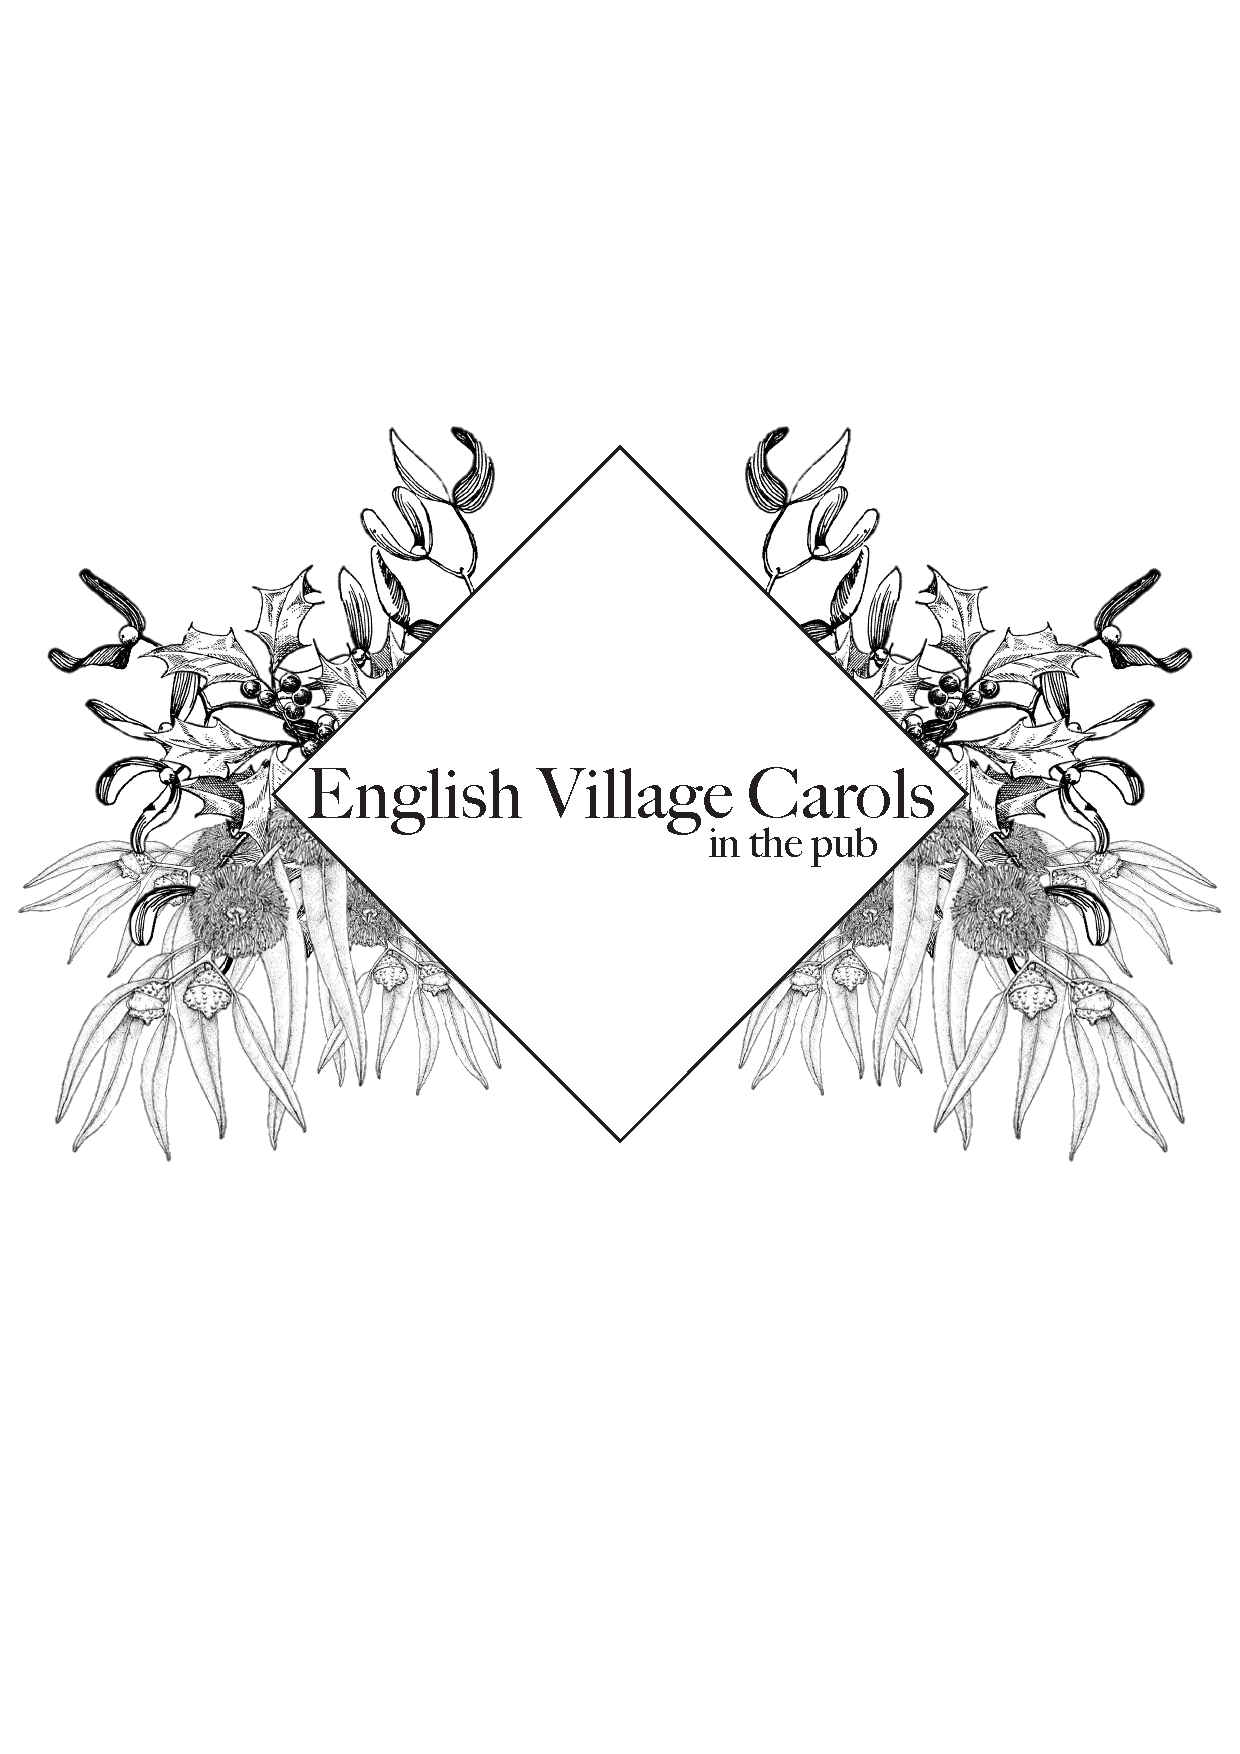
\includepdf[pages=-,pagecommand={\thispagestyle{empty}},scale=0.95,offset=\offset{} 0mm]{./BookCover/cover-print.pdf}
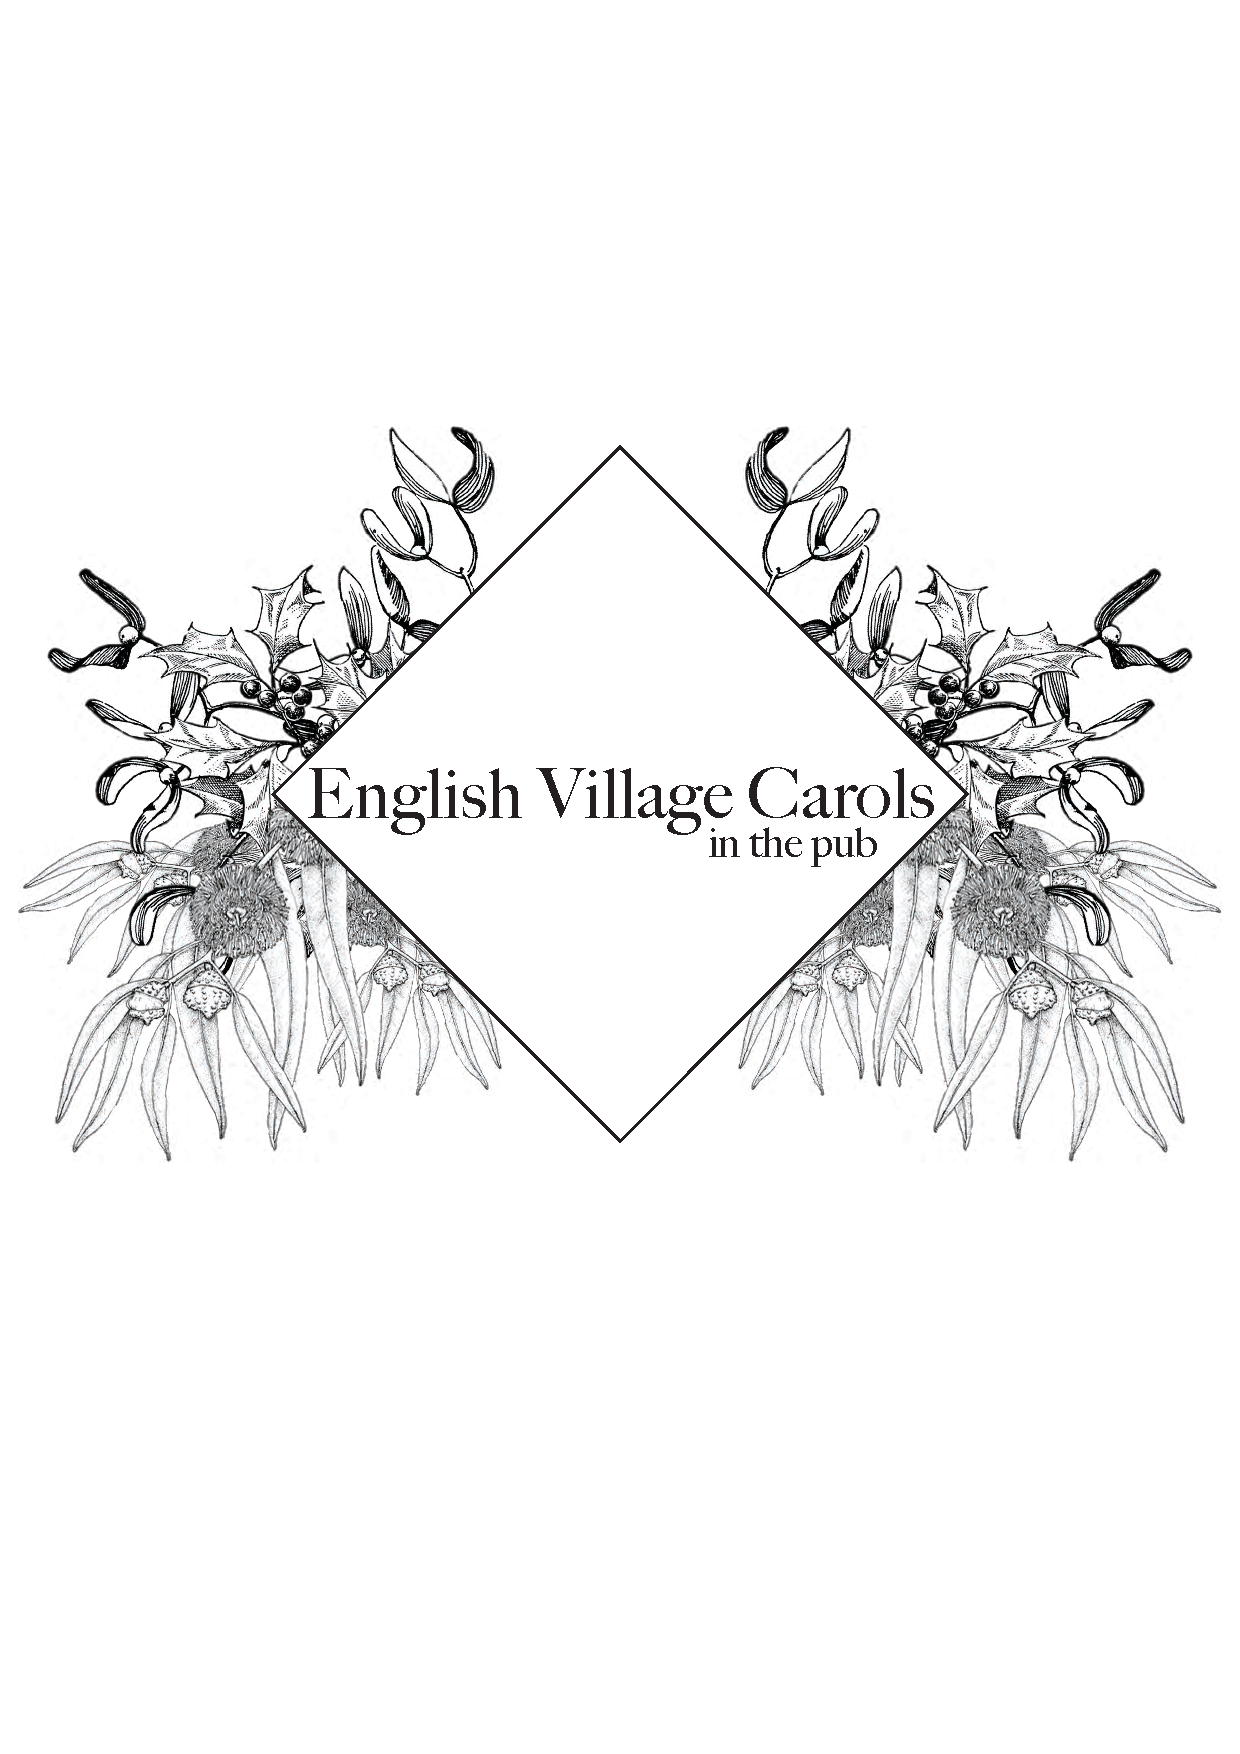
\includepdf[pages=-,pagecommand={\thispagestyle{empty}},scale=0.95,offset=\offset{} 0mm]{./BookCover/cover-webmed.pdf}
\clearpage

\tableofcontents
    \null\vspace{\stretch {3}}
        \begin{center}
\pagenumbering{arabic}
The arrangements in this book are mainly by Ian Russell and have been generously shared for use in Sydney. Please do not redistribute this text.\\ 
To keep up to date with carol-singings in Sydney, please join our \href{https://www.facebook.com/groups/VillageCarolsSydney/}{Village Carols Sydney} Facebook group.\\
\vspace{\stretch{1}}\null
For more information on the tradition we recommend Ian's books \emph{The Sheffield Book of Village Carols} and \emph{The Derbyshire Book of Village Carols}, available through \url{http://www.villagecarols.org.uk}\\

\vspace{\stretch{1}}\null
Music set by Thomas MacDonald in Lilypond and LaTeX. Cover art by Stephanie Swanson.
       \end{center}
\vspace{\stretch{3}}\null


\clearpage

% TWo-page songs should begin on even page numbers (lefthand side) wherever possible.
\addsong{Awake and Arise}{awake_and_arise}

\addsong{Awake, Arise, Good Christians!}{awake_arise_good_christians}

\addsong{Back Lane}{back_lane}

\addsong{The Christmas Tree}{christmas_tree}

\addsong{Curly Hark}{curly_hark}

\addsong{Diadem}{diadem}

\addsong{Egypt}{Egypt}

\addsong{Good News}{good_news}

\addsong{Hail! Chime on}{hail_chime_on}

\addsong{Hail, Smiling Morn!}{hail_smiling_morn}

\addsong{Hark Hark, Hark Hark}{hark_hark}

\addsong{How Beautiful Upon The Mountains}{how_beautiful_upon_the_mountain}

\addsong{Jacob's Well}{jacobs_well}

\addsong{Little Bilberry}{little_bilberry}

\addsong{Liverpool}{liverpool}

\addsong{Lloyd}{lloyd}

\addsong{Lo, the Eastern Magi Rise}{lo_the_eastern_magi_rise}

\addsong{Malin Bridge}{malin_bridge}

\addsong{Merry Christmas}{merry_christmas}

\addsong{The Mistletoe Bough}{mistletoe_bough}

\addsong{Mount Moriah}{mount_moriah}

\addsong{Mount Zion}{mount_zion}

\addsong{Old Foster}{old_foster}

\addsong{Peace O'er the World}{peace_oer_the_world}

\addsong{Pentonville}{pentonville}

\addsong{Prodigal Son}{prodigal_son}

\addsong{Reapers}{ho_reapers}

\addsong{Rolling Downward}{rolling_downward}

\addsong{Shepherds Arise}{shepherds_arise}

\addsong{Shepherds Rejoice}{shepherds_rejoice}

\addsong{Spout Cottage}{spout_cottage}

\addsong{Stannington}{stannington}

\addsong{Star of Bethlehem}{star_of_bethlehem}

\addsong{Sweet Chiming Bells}{sweet_chiming_bells}

\addsong{Tinwood}{tinwood}

\addsong{Tyre Mill}{tyre-mill}

\clearpage

\section*{Versions of this book}
\subsection*{First printing (2018)}
\begin{itemize}
    \item 31 songs over 52 pages.
    \item Song ordering largely alphabetical but with some fudging to keep 2-page songs on facing pages.
\end{itemize}
\subsection*{Second printing (2022)}
\begin{itemize}
    \item Multiple fixes of typos and incorrect word alignment below music.
    \item Song ordering changed to be fully alphabetical. 
    \item Added: Hail Chime On, Reapers, Shepherds Arise, Stannington, Tyre Mill. 36 songs over 56 pages.
\end{itemize} 

\end{document}

